\documentclass[a4paper,11pt]{article}
\usepackage{configuration}


\begin{document}
%\begin{titlepage}
 \thispagestyle{empty}
\begin{center}
 
\textsc{\LARGE Université de Mons-Hainaut}\\[0.5cm]
\textsc{\Large Faculté des Sciences}\\[4.0cm]
\textsc{\Large Simulation de systèmes à évènements discrets}\\[0.5cm]
 
 
% titre
\HRule \\[0.4cm]
{ \Large \bfseries Rapport du projet}\\[0.3cm]
 
\HRule \\[1.5cm]
 
% auteur et directeur
\begin{minipage}{0.4\textwidth}
\begin{flushleft} \large
\emph{Auteurs:} 
\\ Sébastien \textsc{Dubois}
\\ Jean-François \textsc{Mernier}
\\ Frédéric \textsc{Regnier}

\end{flushleft}
\end{minipage}
\begin{minipage}{0.4\textwidth}
\begin{flushright} \large
%\emph{Directeur:} \\ Olivier \textsc{Markowitch}
\end{flushright}
\end{minipage}


% remplit la page (de vide :p)
\vfill

% date avec un peu d'espace ensuite
{\Large \today}\\[1.5cm]

% logos en bas de page

\includegraphics[scale=0.03]{umh/logo-acwalbxl.png}

\includegraphics[scale=0.08]{umh/logo-umh.png}

\end{center}


% ajoute une page vierge après la page de garde
\newpage
\thispagestyle{empty}
\mbox{}
\newpage
%\end{titlepage}

\tableofcontents % table des matières
\pagebreak
\listoffigures % liste des figures
\pagebreak
%\listoftables % liste des tables
%\pagebreak


\section{Evenements}

\subsection{Hotes}
\subsubsection{Envoi d'un message original}
\subsubsection{Réception d'un message}
\subsubsection{Fin de traitement d'un message}
\subsubsection{Timeout}

\subsection{Agents}
\subsubsection{Réception d'un message}
Dans le diagramme UML, il y a deux points que nous n'avons pas expliqué. Tout d'abord: \og Est-ce qu'on peut envoyer les nouvelles informations de routage maintenant? \fg. En fait nous avons décidé d'éviter trop d'envois successifs inutiles d'informations de routage, afin de ne pas surcharger le système. Pour ce faire, quand on doit envoyer les informations de routage (à cause du niveau d'occupation du buffer), on vérifie si ça fait au moins $x$ temps de simulation qu'on a envoyé un message. Si oui, alors on peut envoyer le message. De cette manière, si pour un temps $t$ donné, l'agent reçoit $50$ messages, que pour le premier il dépasse le seuil d'alerte d'occupation du buffer et envoie ses informations de routage, puisqu'il sera toujours au delà du seuil d'alerte pour les $49$ autres messages, on évite ainsi de réenvoyer les informations inutilement.

Le second point: \og Augmentation du coût de nos routes à destination des autres agents (on augmente d'une valeur fixe à chaque fois) \fg est ce que le distance vector prenne en compte le niveau d'occupation des agents. Quand un agent donné est surchargé, il augmente le coût de ses routes à destination d'autres agents et prévient ses voisins. De cette manière quand les voisins reçoivent les informations, ils mettent à jour leur propre DV et choisissent peut être d'autres routes pour faire suivre les messages (sauf si l'agent est la destination finale bien sûr!). Si les autres agents deviennent surchargés, leurs coûts augmenteront également. Ainsi au final, le Dv prend en compte l'occupation des buffers des agents, ce qui permet de mieux répartir la charge sur les différents agents. Dans les résultats des simulations, nous avons observé une bien meilleure répartition.


\subsubsection{Fin de traitement d'un message}
\subsubsection{Envoi des informations de routage}
\subsubsection{Réception d'informations de routage}


\section{Résultats}
\subsection{Paramètres du système}

\subsubsection{Hote}
\begin{itemize}
 \item Durée du timeout (temps après lequel on réémet un message)
 \item Temps maximal inter-envois (pour les messages originaux)
 \item Temps de traitement d'un message
 \item Pourcentage de messages à destination d'un autre agent
\end{itemize}


\subsubsection{Agent}

\begin{itemize}
 \item Nombre d'hôtes reliés
 \item Taux de pertes brutales de messages
 \item Temps de traitement d'un message
 \item Taille de buffer (en entrée)
\end{itemize}

Pour le distance vector on a en plus:
\begin{itemize}
 \item Temps inter-envois des informations de routage
\end{itemize}

\subsubsection{Simulation}
\begin{itemize}
 \item Durée
 \item Délai agent <-> hôte
 \item Distance vector activé (oui/non)
 \item Durée de la période d'initialisation
 \item Périodicité d'affichage des statistiques (e.g., tous les 1\% de simulation)
\end{itemize}



\section{Décisions}

\subsection{Gestion des évènements}
Nous avons choisi d'utiliser une seule FEL pour la simulation. On y place tous les évènements. De plus, pour un temps $t$ de simulation donné, nous avons décidé de traiter certains évènements prioritairement.

\begin{itemize}
 \item En premier lieu on traite les évènements de réception d'informations de routage
 \item Ensuite on traite les évènements de réception d'informations de routage
 \item Ensuite on traite les évènements de réception de messages (accusés et messages normaux)
 \item Ensuite on traite les évènements de timeout (un message pour lequel on a pas encore reçu d'accusé)
\end{itemize}

TODO ajouter explication pour la fin de simulation quand on aura pris une décision!


\subsection{Distance vector}
Nous avons choisi de modifier les coûts en fonction du taux d'occupation du buffer de l'agent. Pour ce faire

TODO continuer


%\pagebreak
\clearpage

%\backmatter % pour ne pas numéroter à la fin
\appendix

\section{Le programme et son utilisation}
L'exécutable du projet est disponible dans le dossier \textbf{target/dist}. Pour l'exécuter, il suffit d'ouvrir un prompt et de lancer: \textbf{java -jar simulation.jar}.

\subsection{Configuration et aide}
Pour afficher la liste des paramètres pouvant être donnés au programme, il suffit d'ouvrir un prompt et de lancer: \textbf{java -jar simulation.jar --aide}


\begin{figure}[h!t]
  \centering
    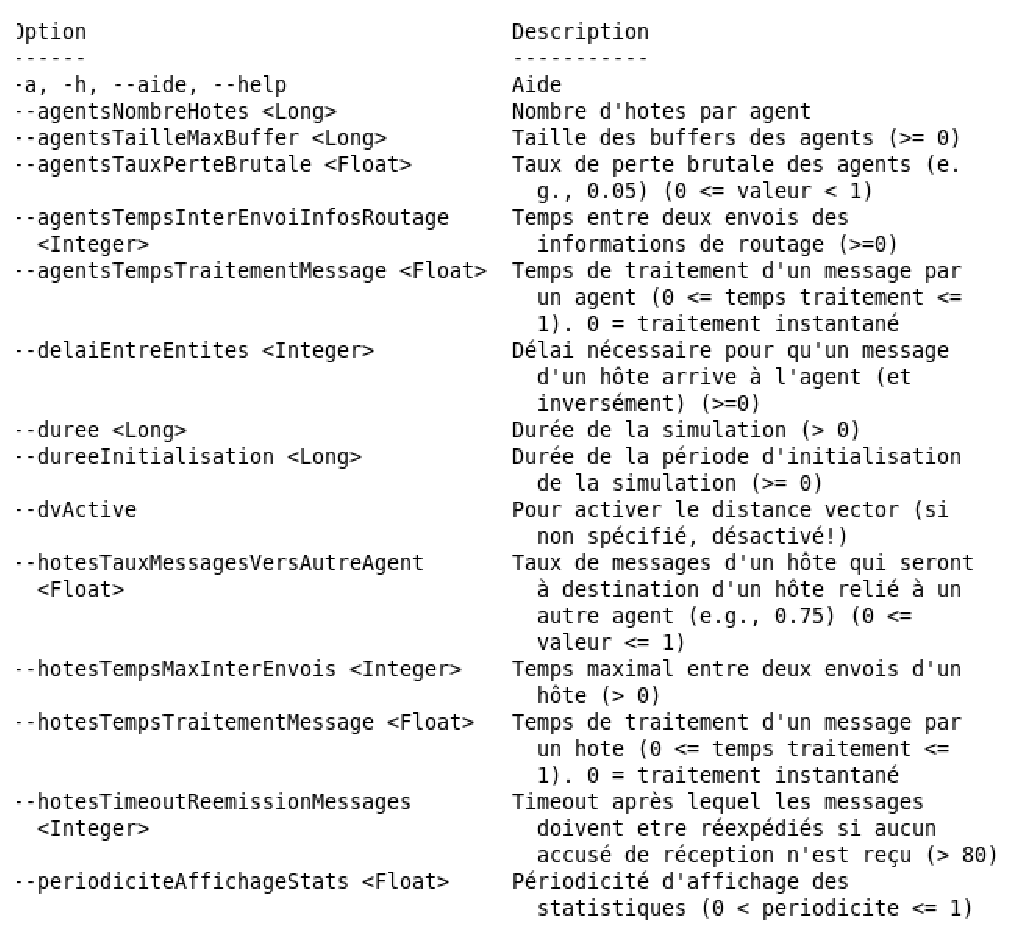
\includegraphics[scale=0.65]{options.eps}
  \caption{Options disponibles}
  \label{fig:options}
\end{figure}

Ensuite pour spécifier les options, on peut par exemple faire: \textbf{java -jar simulation.jar --agentNombreHotes 1000 --duree 5000}.

\subsection{Organisation du code source}
\begin{itemize}
 \item Les sources se trouvent dans le dossier \textbf{src/main/java}
 \item Les fichiers de configuration par défaut se trouvent dans le dossier \textbf{src/main/resources/configuration}
\end{itemize}

Le point d'entrée du programme est la classe \textit{Main} qui se trouve dans \textbf{src/main/java/be/simulation}.

\subsection{Exécution de la simulation}
Lancer le programme exécute directement la simulation. Si aucune option n'est spécifiée en argument au programme, les valeurs par défaut sont utilisées. Les résultats sont affichés à l'écran et sauvegardés dans un fichier de log.

\subsection{Compilation}
La compilation du code requiert l'utilisation de Maven \footnote{\url{http://maven.apache.org/}}, un outil de build très simple d'utilisation. En étant dans le dossier du projet (au niveau où se trouve le fichier \textbf{pom.xml}), il suffit d'exécuter la commande suivante: \textbf{mvn package}. Une fois terminé, le fichier jar exécutable est disponible dans le dossier \textbf{target/dist}.

Maven est très simple à installer sur la plupart des distributions Linux (e.g., Ubuntu, ...). Sous Windows, il suffit de le télécharger et d'ajouter le dossier bin au path.



\subsection{UML}
Un diagramme de classes montrant les classes principales du projet existe mais n'a pas été inclus dans le rapport car il est trop grand. Il est disponible dans le dossier \textbf{UML} qui accompagne le rapport (le fichier: \textbf{CD Entites.png}).
\appendix



\end{document}
